% Use only LaTeX2e, calling the article.cls class and 12-point type.

\documentclass[11pt]{article}

\usepackage[round,semicolon]{natbib}
\usepackage{etoolbox}
\AtBeginEnvironment{quote}{\singlespacing\tiny}
% Use times if you have the font installed; otherwise, comment out the
% following line.

% added by SKH
\usepackage{lineno}
%\linenumbers

\usepackage{times}
\usepackage{amssymb}
\usepackage{amsmath}

\usepackage[export]{adjustbox}

\usepackage{graphicx}
\graphicspath{ {images/} }

% for adjustwidth
\usepackage{changepage}

% The following parameters seem to provide a reasonable page setup.

\topmargin 0.0cm
\oddsidemargin 1cm
\textwidth 15cm 
\textheight 21cm
\footskip 1.0cm

\usepackage{newfloat}
\usepackage{amsmath}
\usepackage[labelfont=bf]{caption}
\usepackage{nameref}
\usepackage{rotating}
\usepackage{color}
\usepackage{float}

% allow bigger floats per here: https://tex.stackexchange.com/a/11382
\renewcommand{\topfraction}{.95}
\renewcommand{\bottomfraction}{.95}
\renewcommand{\textfraction}{.05}
\renewcommand{\floatpagefraction}{.95}
\renewcommand{\dbltopfraction}{.66}
\renewcommand{\dblfloatpagefraction}{.66}
\setcounter{topnumber}{9}
\setcounter{bottomnumber}{9}
\setcounter{totalnumber}{20}
\setcounter{dbltopnumber}{9}

\renewcommand{\figurename}{{}}
\renewcommand{\thefigure}{{Figure~\arabic{figure}}}

\renewcommand{\tablename}{{}}
\renewcommand{\thetable}{{Table~\arabic{table}}}

\newfloat{suppfile}{thp}{losuppfile}
\renewcommand{\thesuppfile}{Supplementary~file~\arabic{suppfile}}
\floatname{suppfile}{}

\newfloat{suppfig}{thp}{losuppfig}
\renewcommand{\thesuppfig}{Supplementary~figure~\arabic{suppfig}}
\floatname{suppfig}{}

%
\newfloat{supptable}{thp}{losupptable}
\renewcommand{\thesupptable}{Supplementary~table~\arabic{supptable}}
\floatname{supptable}{}
%

\renewcommand{\theequation}{Equation~\arabic{equation}}

\newcommand\skhcomment[1]{{\color{cyan}[#1]}}
\newcommand\jdbcomment[1]{{\color{red}[#1]}}


\usepackage{hyperref}
\hypersetup{colorlinks,citecolor=blue,linkcolor=blue,urlcolor=blue}
\hypersetup{colorlinks,citecolor=blue,linkcolor=blue,urlcolor=blue}

\usepackage{seqsplit}

\usepackage{array}
\newcolumntype{P}[1]{>{\raggedright\arraybackslash}p{#1}}

\title{A Susceptible-Infected-Vaccinated Model for Influenza Infection Dynamics} 

\author
{Jonathan Mah$^{1*}$\\
\\
\footnotesize{$^1$College of Arts \& Sciences, University of Washington}\\
\footnotesize{Seattle, WA}\\
\footnotesize{$^*$AMATH 383: Introduction to Continuous Modeling}\\
}


% Include the date command, but leave its argument blank.

\date{}

\usepackage{setspace}
\onehalfspacing


\begin{document} 

% Make the title.

\maketitle 


\begin{abstract}
\noindent  
A current problem in public health is our inability to reliably forecast the timing and intensity of seasonal Influenza. Current models for infectious diseases like SIR (susceptible-infected-vaccinated) models inadequately account for the seasonal dynamics of Influenza and the time-limited effectiveness of vaccination. In this work, we propose an SIV (susceptible-infected-vaccinated) model which takes into account both the seasonal pattern of Influenza outbreaks as well as the time-limited effectiveness of vaccinations. Additionally, we use relevant clinical and epidemiological data to inform the choice of model parameters. Given sufficiently informed parameters, the SIV model may provide insight towards the behavior of influenza outbreaks, however, further work is necessary for accurate prediction of infection dynamics.
\end{abstract}

\clearpage

\section*{Problem Description} 

The goal of this project is to expand upon existing epidemiological models for infection dynamics. One such model, the SIR model, separates the population into three disjoint sets, being ``\textbf{S}usceptible", ``\textbf{I}nfected", and ``\textbf{R}ecovered". The SIR model is given by the following system of differential equations:
\begin{equation} \label{SIR}
\begin{aligned}
\frac{dS}{dt} &= -\alpha I S \\
\frac{dI}{dt} &= \alpha I S - \beta I \\
\frac{dR}{dt} &= \beta I 
\end{aligned}
\end{equation}
where $\alpha$ represents the rate of infection and $\beta$ represents the rate of recovery. This model makes a few key assumptions. One such assumption is that the total population remains constant. Note that the sum of derivatives, $\frac{dS}{dt} + \frac{dI}{dt} + \frac{dR}{dt} = 0$, which implies that the derivative of the sum is also equal to $0$. Thus, the total population does not change. 

Another key assumption is that individuals stay ``Recovered", making this an absorbing state. Given parameters $\alpha = 0.004$ and $\beta = 1$, with initial conditions $S = 999$, $I = 1$, $R = 0$, we find that the SIR model follows the following density distribution, eventually reaching equilibrium.
\begin{center}
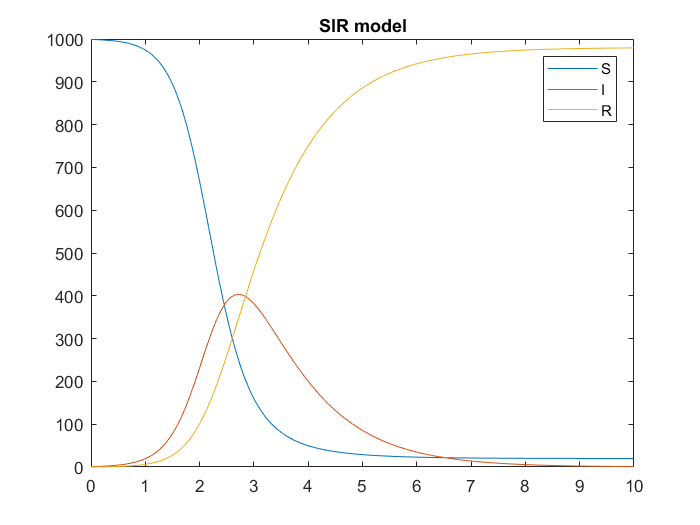
\includegraphics[scale=0.7]{../Data/sirModel.png}
\end{center}
While possibly appropriate for certain diseases like chicken pox, the SIR model fails to take into account the ability of certain viruses to escape the immune response. Additionally, the SIR model is blind to time -- only the current state is taken into consideration. As a result, the SIR model is unsuitable for modeling the infection dynamics of diseases like Influenza, which is well known for being able to escape the human immune response and for having seasonal outbreaks.

\section*{Simplifications}

\section*{Mathematical Model}

\section*{Solution of the Mathematical Problem}

\section*{Results and Discussion}

\section*{Improvement}

\section*{Conclusions}

\clearpage 
\bibliographystyle{mbe}
{\small
\bibliography{references.bib}
}


\end{document}